%!TEX program = xelatex
% not lualatex because of a pgf bug: https://sourceforge.net/p/pgf/bugs/384/
\documentclass[12pt, a4paper]{report}
\usepackage[T1]{fontenc}
\usepackage[french]{babel}
\usepackage{hyperref}
\usepackage{utbmcovers}
\usepackage{hyphenat}
\usepackage[scale=0.7]{geometry}

%----------------------------------------
% hyperref configuration
%----------------------------------------

\hypersetup{
    colorlinks=true,
    urlcolor=,
}

\graphicspath{{images/}}

\newcommand\tab[1][1cm]{\hspace*{#1}}
\newcommand\TODO[1]{\textcolor{red}{TODO\@: #1}}

%----------------------------------------
% utbmcovers configuration
%----------------------------------------

\setutbmfrontillustration{utbm_default_illustration}
\setutbmtitle{Développement d’une plateforme de recueuil de consentements RGPD}
\setutbmsubtitle{Rapport de stage ST50 \hyp{} A2019}
\setutbmstudent{Nicolas BALLET}
\setutbmstudentdepartment{Département Génie Informatique}
\setutbmstudentpathway{Filière libre}
\setutbmcompany{Entreprise Versusmind}
\setutbmcompanyaddress{30 avenue du Rhin\\ 67000 Strasbourg}
\setutbmcompanywebsite{\href{versusmind.eu}{versusmind.eu}}
\setutbmcompanytutor{Philippe Didiergeorges}
\setutbmschooltutor{Vincent Hilaire}
\setutbmkeywords{RGPD \hyp{} Consentement \hyp{} Signature numérique \hyp{} Plateforme Azure \hyp{} Méthodologie Scrum \hyp{} Cloud \newline Angular \hyp{} Spring Boot \hyp{} Azure Functions}
\setutbmabstract{<RÉSUMÉ>}

%----------------------------------------
% document
%----------------------------------------

\begin{document}
	\makeutbmfrontcover{}
        \TODO{Je tiens tout d'abord à remercier\ldots}
    \newpage
    \tableofcontents
    \chapter{Introduction}
        \section{Entreprise}
            \tab{} Versusmind est une entreprise de consultation informatique, elle est découpée en plusieurs agences, Nancy (centre), Metz, Strasbourg, Paris, Luxembourg.\newline
            Elle compte aujourd'hui X employés. Elle fournit aux entreprises une expertise ainsi que la réalisation leurs projets.
            \TODO{}
        \section{Projet}
            \subsection{Contexte}
                \tab{} Adopté par l’Union Européenne en avril 2016, la date d’application du RGPD est le 25 mai 2018. Celui-ci oblige les entreprises à identifier les données personnelles en leur possession ainsi que leurs modalités de traitement et de protection et a pour objectifs de\@:
                \begin{enumerate}
                    \item Uniformiser la réglementation au niveau européen
                    \item Responsabiliser les entreprises
                    \item Renforcer les droits des personnes
                \end{enumerate}
                \tab{} Le non-respect du RGPD peut mener à des sanctions financières importantes ainsi qu'a des sanctions administratives ayant un fort impacte sur le fonctionnement de l'entreprise.
                Il est donc important pour les entreprises d'être en conformité avec le RGPD.\newline
                Mais faire migrer son système d'information pouvant coûter cher, Versusmind propose une solution nommée Central Consent Manager.
            \subsection{Central Consent Manager (CCM)}
                \tab{} CCM est système de gestion des consentements centralisé qui va permettre aux entreprises de se libérer d'un poids en s'assurant que ses utilisateurs ont bien consentis à l'utilisation de leurs données personnelles en centralisant l'enregistrement et la vérification d'authenticité des consentements.\newline
                \begin{center}
                    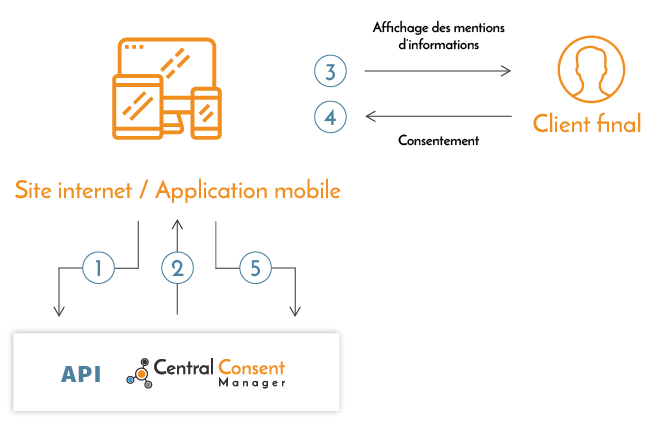
\includegraphics[width=0.8\textwidth]{ccm.png}
                \end{center}
                \begin{enumerate}
                    \item Requête sur le service de mentions pour un traitement
                    \item Envoi des mentions d'informations
                    \item Envoi d'un e-mail de confirmation (vérification d'identité minimale)
                    \item Confirmation
                    \item Enregistrement du consentement
                \end{enumerate}
            \subsection{Ma mission}
                \tab{} Dans une équipe de développeurs qui évolue beaucoup, mon rôle a été d'aider au développement de la plateforme CCM, à sa mise en production et à améliorer ses performances.\newline
                \TODO{}
    \chapter{Développement}
        \section{Méthodologie Scrum}
            J'ai été intégré durant mon stage à une équipe utilisant la méthodologie Scrum, qui fait partie des méthodes de gestion de projet agiles. Cela vise à supprimer ou au moins à réduire l'effet tunnel d'une méthode de gestion classique.\newline
            Le développement est découpé en cycles (de trois semaines dans le cas présent) que l'on appelle ``sprint``.\newline
            Au lieu d'un cahier des charges donné au début du projet, on va le découper en scénarios tout au long du projet avec l'aide du client.\newline
            Cela permet de rester concentré sur les aspects importants et de ne pas développer de fonctionnalités qui ne seront jamais utilisées.\newline
            Un Scrum Master est assigné au projet, son rôle est d'aider l'équipe à bien suivre un fonctionnement agile ainsi qu'a s'organiser, il est aussi là pour guider le client dans la rédaction des scénarios.
            \begin{center}
                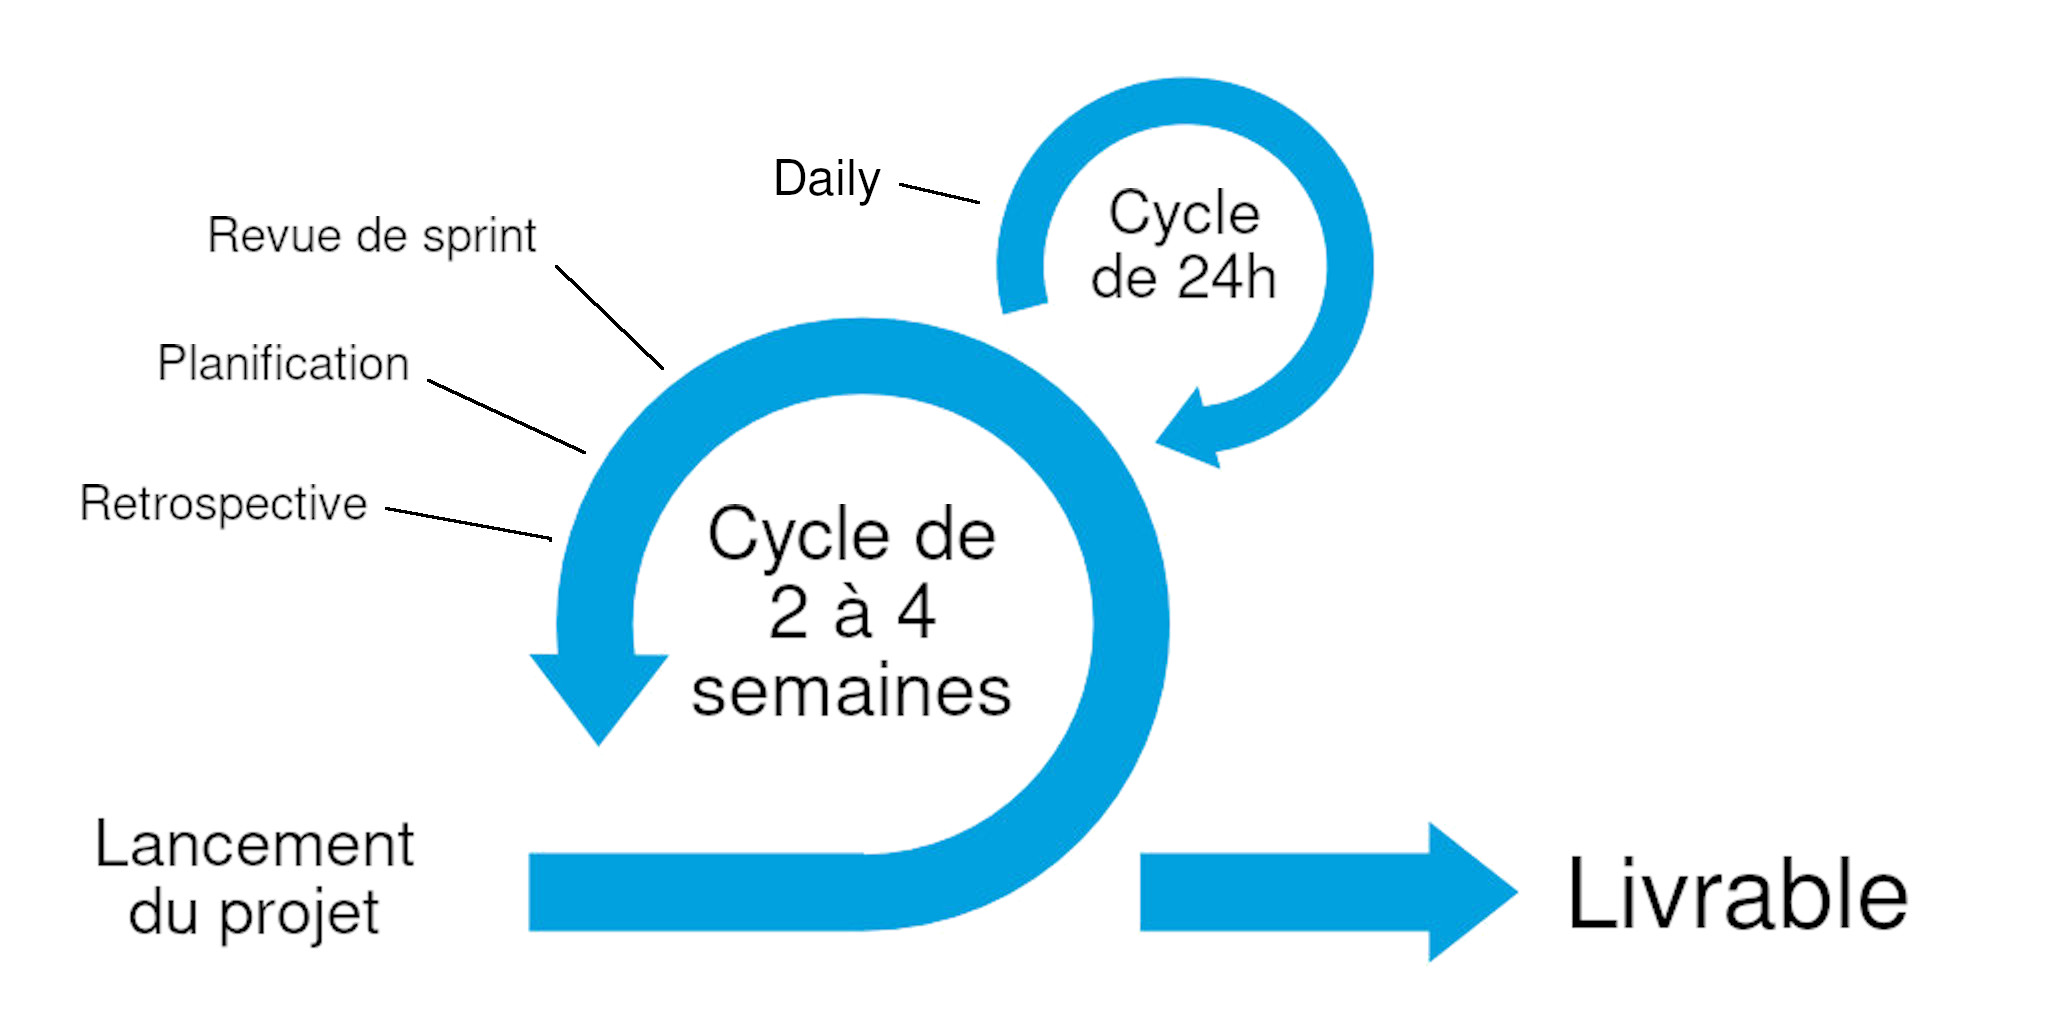
\includegraphics[width=\textwidth]{scrum.jpg}
            \end{center}
            \subsection{Réunions journalières (Daily)}
                Chaque matin nous avions une petite réunion qui ne doit pas dépasser 15min afin d'informer rapidement le reste de l'équipe de l'avancement des différentes taches, de discuter brièvement des différents problèmes rencontrés mais aussi de choisir ensemble la priorité des différentes taches qu'il reste à faire.\newline
                Cela permet de rester toujours conscient de l'état du projet et d'avoir une vision d'ensemble du travail accompli et du travail restant.
            \subsection{Réunions inter-sprints}
                Entre chaque sprint, une série de réunions nous permet de rester dans la bonne direction concernant le développement du projet.
                \subsubsection{Revue de sprint}
                    Le but de la revue de sprint est de montrer à toutes les parties prenantes l'avancement du projet pendant le dernier sprint.\newline
                    Une fois une explication claire du travail accompli et après une démonstration du résultat, on discute afin de peut-être corriger la direction à prendre pour le prochain sprint.
                \subsubsection{Planification}
                    S'en suit la planification, elle se fait avec le Scrum Master ainsi que les développeurs.\newline
                    On va y sélectionner les scénarios à implémenter durant le prochain sprint. Cela constituera ce qu'on appelle ``L'objectif de sprint``.\newline
                    Sous forme d'un nombre on va se mettre d'accord sur une complexité pour chaque scénarios. Cela permet de vérifier qu'on en à bien la même compréhension. Si je propose 1 (facile) et qu'un de mes collègue propose 4 (moyen), c'est que l'un de nous deux à mal compris ce qui est attendu.\newline
                    Ensuite on découpe chaque scénarios en taches concrètes et enfin on estime le temps de travail sur chaque taches.
                \subsubsection{Rétrospective}
                    Et enfin, encore une fois avec le Scrum Master ainsi que les développeurs, on discute de comment s'est déroulé le dernier sprint, des pratiques qu'on pourrait mettre en place ou améliorer, mais aussi de comment on l'a vécu et ressenti.\newline
                    Cela s'inscrit dans un objectif d'amélioration de l'environnement de travail et de l'efficacité.
        \section{Développement dirigé par les tests (TDD)}
            Durant mon stage, j'ai appris à implémenter des tests afin de subvenir à plusieurs besoins\@:
            \begin{enumerate}
                \item Fournir une preuve de fonctionnement du code testé
                \item Prévenir d'éventuels bugs futurs
                \item S'assurer du bon fonctionnement de l'application avant son déploiement
            \end{enumerate}
            Afin de s'assurer de cela, on a défini le comportement unitaire de chaque composant, ainsi qu'un ou plusieurs parcours d'utilisation critiques utilisant les éléments clés de l'application.\newline
            Et dans une démarche d'intégration continue j'ai participé à la mise en place de systèmes de tests et de déploiement automatisés sur la plateforme Azure.\newline
                J'ai pu utiliser la solution SonarQube qui s'occupe d'analyser le dépôt de code source afin d'y trouver des problèmes de sécurité, des bugs, des mauvaises pratique ainsi que de la duplication de code.\newline
                Cela contribue a rendre le code plus stable et plus maintenable.\newline
                J'ai eu l'occasion de créer différents types de tests\@:
                \begin{description}
                    \item [Les tests unitaires] s'assurent que chaque composant de l'application rempli son rôle.
                    \item [Les tests d'intégrations] vérifient un fonctionnement comportant plusieurs composants.
                    \item [Les test de bout en bout] implémentent des scénario complet, utilisant toutes les couches de l'application.
                \end{description}
        \section{Architecture}
            \TODO{<Inserer le schéma global>}
            \subsection{Front-end}
                \tab{} Je suis arrivé sur la fin d'une saison de refonte graphique.
                J'ai commencé mon stage en me formant sur l'utilisation du framework Angular sur lequel je suis maintenant à l'aise.
                J'ai pu ensuite aider à la fermeture de cette saison en apportant mes connaissances et mon expérience à l'équipe.\newline
                Aussi, tout au long de mon stage, j'ai pu faire de la veille et guider l'équipe vers une restructuration de l'architecture CSS plus maintenable et plus facile à étendre.
            \subsection{Back-end}
                J'ai contribué au développement du back-end du projet, sous forme d'ajout de fonctionnalités, correction de faille de sécurité, correction de bugs, etc\ldots\newline
                Le back-end est un serveur web développé avec Java Spring Boot. Il est le point central de l'application car au cœur de l'architecture.
            \subsection{Gestion du cache}
                Je n'ai pas touché au développement de la gestion du cache côté serveur, mais j'ai participé aux discussions et aidé à la prise de décisions.
                Nous avons opté pour l'utilisation d'un serveur Redis, qui stocke des paires clé-valeur de manière très rapide.\newline
                Nous avons fait face à un problème de mise à jour des données présentes à la fois dans la base de données et dans le cache. La solution vers laquelle nous nous somme orientés est de simplifier les requêtes faites en base pour unifier la récupération des données (abstraire le cache et la base de données) et de filtrer les données dans une couche applicative.
            \subsection{Certification numérique}
                Dans l'objectif d'enregistrer des consentements et de pouvoir justifier leurs validité, nous avons choisi d'utiliser EJBCA qui est une solution auto-hébergée d'autorité de certification.\newline
                Pour chaque nouveau consentement on commence par générer une paire de clé, la clé privée va servir à signer le consentement et ensuite la clé publique sera signée par notre instance EJBCA.\newline
                Lors de la vérification on va récupérer la clé publique signée par EBJCA, effectuer à nouveau la signature du consentement, et vérifier que la signature correspond bien à la signature que l'on à reçu lors de la création du consentement.\newline
            \subsection{Montée en charge}
                \tab{} Suite à la refonte graphique, nous sommes entrés dans une saison de mise en production.\newline
                Une problématique de performances est apparue assez vite. Lorsqu'un nouveau client veux migrer vers CCM, une base de consentements potentiellement conséquente doit être importée. \newline
                Suite à des tests de charge, nous avons observer qu'il faudrait environ 3 jours pour importer une base d'un million de consentements. Et plusieurs heures pour générer un export des consentements enregistrés. Ce n'était pas acceptable.\newline
                J'ai eu la responsabilité d'implémenter des fonctions Azure en Java afin de paralléliser chaque création de signature numérique.
                Afin d'interconnecter le back-end et les fonctions Azure nous avons choisi d'utiliser des Service Bus qui sont de simple files d'attentes de messages formatés en JSON.\newline
                On sérialise les consentements avant les envoyer, il seront désérialisés en arrivant dans la fonction Azure, et la même chose se produira dans l'autre sens une fois la signature récupérée pour être enregistrée en base par le back-end.\newline

                Le fait de paralléliser les traitements nous offre une puissance explosive, plus le nombre de requêtes augmente, plus il y a de serveurs dynamiquement déployés par Azure.\newline
    \chapter{Conclusion}
        \TODO{}
	\makeutbmbackcover{}
\end{document}
